\documentclass[twoside,11pt]{article}

% nohyperref: avoids hyperref/pdftexcmds.sty on minimal TeX installs.
% Remove nohyperref once texlive-latex-recommended is installed.
\usepackage[preprint,nohyperref]{jmlr2e}
\usepackage{booktabs}
\usepackage{amsmath}
\usepackage{url}
\usepackage{lastpage}
\usepackage{graphicx}
\usepackage{float}

% Submission draft metadata for https://jmlr.csail.mit.edu/manudb/
\jmlrheading{0}{2026}{1-\pageref{LastPage}}{7/26}{--}{--}{Atharv Sharma}

\ShortHeadings{SOPHI: Open End-to-End BEV Driving Stack}{Sharma}
\firstpageno{1}

\begin{document}

\title{SOPHI: An Open End-to-End Camera--LiDAR Planning Stack\\
with Sparse-Convolution Inference for NAVSIM}

\author{\name Atharv Sharma \email atharv228.as@gmail.com}

\editor{TBD}

\maketitle

\begin{abstract}
We release \textbf{SOPHI} (\emph{Sparse-conv Offline Perception with Hydra-distillation Inference}), an open Apache-2.0 software stack for training, evaluating, and deploying an end-to-end autonomous driving planner on NAVSIM. A fused camera--LiDAR bird's-eye-view (BEV) feature $\mathbf{F}_{\mathrm{env}}$ is shared by a Hydra-MDP-style trajectory decoder and auxiliary 3D detection and BEV segmentation heads. NVIDIA's CUDA-BEVFusion reference provides a high-performance detection runtime but ships a closed LiDAR sparse-convolution (SCN) binary and omits segmentation and planning. SOPHI replaces that closed SCN path with open \texttt{spconv}~2.x, exports the full multi-head graph to ONNX/TensorRT, and documents a reproducible train$\to$evaluate$\to$export$\to$C++ deploy workflow so others can build their own models. On an RTX~3060 we measure ${\sim}40$\,ms LiDAR SCN latency (${\sim}391$\,ms end-to-end C++ FP16). On the NAVSIM \texttt{navtest} split ($12{,}149$ scenarios) the released checkpoint scores PDM~$0.7925$ (NC~$0.982$, DAC~$0.975$, TTC~$0.981$). Python and C++ trajectories agree to within $1.7$\,mm max absolute error (cosine similarity $1.000$).
\end{abstract}

\begin{keywords}
open source software, autonomous driving, bird's-eye view, sparse convolution, TensorRT, NAVSIM
\end{keywords}

\section{Introduction}
\label{sec:intro}

Learned planners such as Hydra-MDP~\cite{hydramdp2024} and GTRS~\cite{gtrs2024} score a trajectory vocabulary from a dense BEV environment encoding. BEVFusion~\cite{liu2023bevfusion} and NVIDIA's CUDA-BEVFusion~\cite{nvidia2022cudabevfusion} supply a strong camera--LiDAR fusion template for detection, but the reference deployment (i)~depends on a non-redistributable \texttt{libspconv} for the LiDAR SCN, (ii)~exports detection only, and (iii)~does not document a closed loop from NAVSIM~\cite{dauner2024navsim} training through TensorRT planning.

\textbf{SOPHI} fills that gap as \emph{software}, not as a new planning algorithm. We reuse the public BEVFusion backbone and a Hydra-style distillation decoder, and contribute: (1)~an open SCN ONNX executor on \texttt{spconv}~2.x~\cite{spconv2022}; (2)~ONNX/TensorRT export and a C++ runtime for planning, detection, and BEV segmentation on a shared $\mathbf{F}_{\mathrm{env}}$; (3)~a single-environment training and PDM evaluation recipe; (4)~validated navtest scores and Python$\leftrightarrow$C++ parity. The goal is that a researcher can download the stack, retrain or swap heads, and redeploy without the closed SCN binary.

\paragraph{Related software.}
We build on BEVFusion~\cite{liu2023bevfusion}, lift-splat-shoot~\cite{philion2020lss}, SECOND-style sparse ops~\cite{yan2018second}, open \texttt{spconv}~\cite{spconv2022}, Hydra-MDP/GTRS~\cite{hydramdp2024,gtrs2024}, and NAVSIM/PDM~\cite{dauner2024navsim,dauner2023pdm}. Our contribution is the open integration and deployment path.

\section{Software Overview}
\label{sec:software}

\begin{figure}[t]
  \centering
  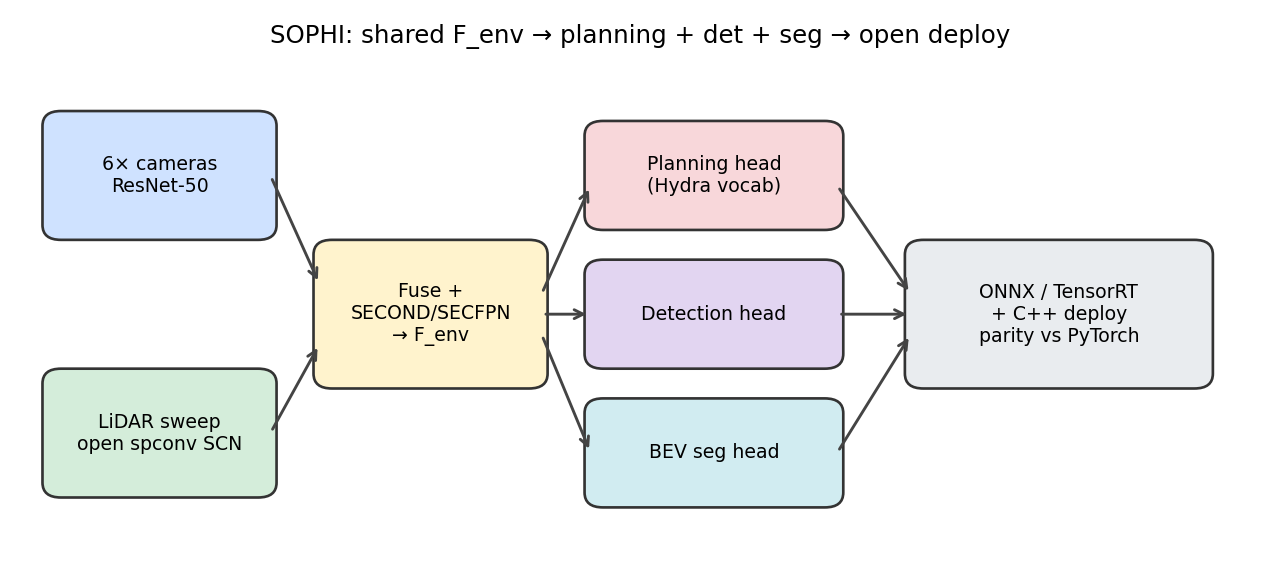
\includegraphics[width=\linewidth]{figures/architecture_pipeline.png}
  \caption{SOPHI layout. Camera (ResNet-50/LSS) and open-\texttt{spconv} LiDAR SCN fuse into $\mathbf{F}_{\mathrm{env}}$, consumed by planning, detection, and BEV-segmentation heads. TensorRT runs dense graphs; SCN runs via the open parser.}
  \label{fig:arch}
\end{figure}

\paragraph{Repository layout.}
The release (Apache-2.0) is at \url{https://github.com/atharvsharma1998/hydra-mdp}
(tag \texttt{v0.1.0-mloss}): \texttt{navsim/agents/gtrs\_bevfusion/} (model/losses),
\texttt{scripts/training/train\_gtrs\_bevfusion.py},
\texttt{scripts/export/export\_gtrs\_bevfusion\_onnx.py}, and
\texttt{deploy/} (C++/TensorRT~\cite{tensorrt2023} + parity).
\texttt{REPRODUCIBILITY.md} lists copy-paste commands for each step below.

\paragraph{Architecture.}
Camera images and a LiDAR sweep produce $\mathbf{F}_{\mathrm{env}}\in\mathbb{R}^{512\times H\times W}$ via LSS view transform~\cite{philion2020lss}, voxel SCN, convolutional fusion, and a SECOND/SECFPN decoder (Figure~\ref{fig:arch}). $\mathbf{F}_{\mathrm{env}}$ is tokenized and fed to a Transformer trajectory scorer with a frozen vocabulary (up to $K{=}8192$), trained by soft imitation and per-proposal PDM sub-score distillation~\cite{dauner2023pdm}. Auxiliary CenterPoint-style detection and a multiclass BEV segmentation head (class-frequency CE + Lov\'asz-softmax~\cite{berman2018lovasz}) supervise the same feature for representation shaping and debugging; they do not gate the plan.

\paragraph{Open SCN runtime.}
The LiDAR ONNX graph (${\sim}53$ nodes) is executed by \texttt{ONNXLiDARModel}: FP16 KRSC weights on GPU, topological \texttt{spconv}~2.x ops (\texttt{kMaskImplicitGemm} with tuner cache, SubM pair-table reuse, grow-only scratch buffers). This replaces NVIDIA's closed \texttt{libspconv} while preserving the exported graph interface. Dense graphs (camera backbone/vtransform, fuser, planning/det/seg heads) are built with TensorRT~8.6 FP16 engines; the camera ResNet uses FP32 compute with FP16 I/O to avoid overflow.

\section{Reproducibility Workflow}
\label{sec:workflow}

Anyone adapting SOPHI follows five steps (details in \texttt{REPRODUCIBILITY.md}):
(1)~Environment --- Python~3.8, PyTorch~1.10+cu113, \texttt{mmcv-full}~1.4,
OpenMMLab \texttt{mmdet3d} (CUDA-BEVFusion fork), \texttt{spconv}~2.x, TensorRT~8.6;
set \texttt{BEVFUSION\_ROOT}, \texttt{NUPLAN\_MAPS\_ROOT}, \texttt{PYTHONPATH}.
(2)~Data --- download NAVSIM logs/sensors/maps; run \texttt{run\_metric\_caching.py}
with a process pool.
(3)~Train --- \texttt{train\_gtrs\_bevfusion.py} on \texttt{navtrain} (raw model
\texttt{state\_dict}; agent loader strips optional \texttt{agent.}/\texttt{\_model.} prefixes).
(4)~Evaluate --- Hydra agent \texttt{gtrs\_bevfusion\_agent} via \texttt{run\_pdm\_score.py}
on \texttt{navtest} with \texttt{worker.use\_process\_pool=True} (${\sim}10$ workers on an 80\,GB A100).
(5)~Deploy --- export ONNX (\texttt{--lidar-scn}), delete stale \texttt{.plan} files,
\texttt{build\_gtrs\_engines.sh fp16}, run \texttt{gtrs\_bevfusion}, then
\texttt{compare\_cpp\_parity.py}.
An early rasterize-then-plan prototype failed when map thresholds discarded latent
detail; SOPHI therefore plans from tokenized $\mathbf{F}_{\mathrm{env}}$. Map training
uses frequency-weighted CE + Lov\'asz so thin classes are not dominated by road/background.

\section{Experimental Validation}
\label{sec:exp}

\paragraph{Latency (RTX~3060 12\,GB, FP16).}
Table~\ref{tab:latency} reports steady-state C++ timings after open-SCN optimization (20-iteration mean; first-frame tuner warmup excluded). End-to-end wall latency is ${\sim}404$\,ms (${\sim}2.5$\,FPS) on this consumer GPU.

\begin{table}[H]
  \caption{C++ FP16 module latency on RTX~3060 (ms, mean).}
  \label{tab:latency}
  \centering
  \begin{tabular}{lr}
    \toprule
    Module & ms \\
    \midrule
    LiDAR (range-crop + open SCN) & 37.8 \\
    Camera (LSS)                  & 169.8 \\
    Fuser ($\mathbf{F}_{\mathrm{env}}$) & 1.6 \\
    Heads (plan + det + seg)      & 182.2 \\
    \midrule
    \textbf{Total (device)}       & \textbf{391.3} \\
    \bottomrule
  \end{tabular}
\end{table}

\paragraph{NAVSIM navtest PDM.}
On the official single-stage \texttt{navtest} split ($12{,}149$ scenarios; metric cache precomputed), the released checkpoint \texttt{gtrs\_bevfusion\_navtrain\_v1\_best.pth} scores \textbf{PDM $0.7925$}. Stage-one sub-metrics: no-at-fault collision $0.982$, drivable-area compliance $0.975$, driving-direction $0.996$, traffic-light $0.998$, ego progress $0.854$, time-to-collision $0.981$, lane keeping $0.970$, history comfort $0.964$. Safety/compliance are near-saturated; ego progress is the remaining soft spot (conservative plans). Two-stage reactive EPDMS columns are absent because \texttt{navtest} does not ship synthetic reactive frames.

\paragraph{Python$\leftrightarrow$C++ parity.}
On token \texttt{8bc34517e08758ff}, stage-wise cosine similarities are $\ge 0.993$ (Table~\ref{tab:parity}). The deployed trajectory matches PyTorch to $1.7{\times}10^{-3}$\,m max absolute error.

\begin{table}[H]
  \caption{Python vs.\ C++/TensorRT parity (cosine / max$|\Delta|$).}
  \label{tab:parity}
  \centering
  \small
  \begin{tabular}{lcc}
    \toprule
    Stage & Cosine & Max$|\Delta|$ \\
    \midrule
    lidar\_bev / cam\_bev / $\mathbf{F}_{\mathrm{env}}$ & 0.993 / 1.000 / 0.997 & 2.35 / 0.10 / 0.73 \\
    scores / trajectory & 0.9995 / 1.000 & 1.57 / 0.0017 \\
    agent states / class logits & 1.000 / 1.000 & 0.066 / 0.066 \\
    bev\_semantic\_logits & 0.9998 & 1.27 \\
    \bottomrule
  \end{tabular}
\end{table}

\section{Licensing and Limitations}
\label{sec:limits}

\paragraph{What is open.}
Training, export, deploy sources, and documentation are Apache-2.0. Open \texttt{spconv} executes the LiDAR SCN. We build on NVIDIA's Apache-2.0 CUDA-BEVFusion \emph{template} and replace the non-redistributable SCN binary with open inference. We do \emph{not} claim a fully proprietary-free stack: CUDA and TensorRT remain required for the documented C++ path (widely used in the community; justified analogously to other MLOSS GPU libraries). NAVSIM/nuPlan data must be obtained under their own licenses.

\paragraph{Scope.}
SOPHI reuses Hydra-MDP/GTRS scoring and BEVFusion fusion; novelty is the open SCN path, multi-head deploy graph, and end-to-end recipe. PDM~$0.7925$ is competitive but not state-of-the-art (e.g., Transfuser is higher on navtest). Further work includes int8 engines, ego-progress calibration, and two-stage navhard EPDMS.

\section{Conclusion}
\label{sec:conclusion}
SOPHI is an open, documented camera--LiDAR--planning stack for NAVSIM: train multi-task $\mathbf{F}_{\mathrm{env}}$ models, score them with official PDM evaluation, and deploy with open SCN + TensorRT while matching Python trajectories at millimeter scale. We hope it lowers the barrier for researchers who want to modify sparse LiDAR backbones and ship full perception-to-planning runtimes without closed SCN libraries.

\acks{No external funding was received. Source code and the submission archive are released under Apache-2.0 at \url{https://github.com/atharvsharma1998/hydra-mdp} (tag \texttt{v0.1.0-mloss}). Companion instructions: \texttt{jmlr/REPRODUCIBILITY.md}.}

\bibliography{bevfusion_planner}

\end{document}
